\documentclass[xcolor=table]{beamer}
\usepackage[utf8]{inputenc}
\usepackage[spanish]{babel}
\usepackage{listings}
\usepackage{graphicx}
\usepackage{hyperref}
\usepackage[acronym]{glossaries}
\usepackage{appendixnumberbeamer}
\usepackage{caption} % captionof for figures
\usepackage{tikz}
\usetikzlibrary{trees,positioning,arrows}

\tikzstyle{stylepop} = [rectangle, rounded corners, minimum width=1cm, minimum height=2cm,text centered,text width=2.2cm, draw=black, fill=white]
\tikzstyle{arrow} = [thick,->,>=stealth]

\usetheme{Dresden}
\usecolortheme{lily}

\newacronym{hpc}{HPC}{High Performance Computing}
\newacronym{isa}{ISA}{Instruction Set Architecture}
\newacronym{fpga}{FPGA}{Field Programmable Gate Array}
\newacronym{lut}{LUT}{Lock-Up Table}
\newacronym{dsp}{DSP}{Digital Signal Processors}
\newacronym{tlp}{TLP}{Transaction Layer Packet}
\newacronym{axi}{AXI-ST}{AXI4-Stream}
\newacronym{ip}{IP}{Intellectual Property}
\newacronym{vpu}{VPU}{Vector Processor Unit}
\newacronym{rtl}{RTL}{Register-Transfer Level}
\newacronym{dw}{Dword}{Double word}
\newacronym{hdl}{HDL}{Hardware Description Language}


\newacronym{epi}{EPI}{European Processor Iniciative}

\newacronym{io}{IO}{input/ouput}



\title{RISC-V processor in an \acrshort{fpga}}
\author{Jose L. Estragués, Andrea Querol, Guillem Ramírez, Joan Vinyals, Pablo Vizcaino}
\date{May 2021}
\institute[FIB, UPC]{Facultat d'Informàtica de Barcelona \\ Universitat Politècnica de Catalunya - BarcelonaTech \and Barcelona Supercomputing Center}

\setbeamertemplate{page number in head/foot}[totalframenumber]

\AtBeginSection[]
{
  \begin{frame}<beamer>{Outline}
    \tableofcontents[currentsection]
  \end{frame}
}

\newcommand{\aqnote}[1]{ {\color{violet}\textbf{AQ:} #1 } }
\newcommand{\gnunote}[1]{ {\color{blue}\textbf{GNU:} #1 } }

\begin{document}

\begin{frame}
\maketitle
\end{frame}


\begin{frame}{}
    \tableofcontents
\end{frame}

\section{RISCV}
\section{RISC-V}

RISC-V is an open standard instruction set architecture (\gls{isa}) based in the reduced instruction set computer (\gls{risc}) architecture. This architecture is based on a small and highly optimized instructions in contrast with other types of architectures like the complex instruction set computer (\gls{cisc}). The RISC-V \gls{isa} does not need fees to use and several companies and projects  are considering this architecture to develop their products. In addition, open source operating systems with RISC-V support are available and the instruction set is supported in several popular software toolchains. Load-store architecture and IEEE-754 floating point instructions. \\

\subsection{History}

Prof. Krste Asanović and graduate students Yunsup Lee and Andrew Waterman started the RISC-V instruction set in May 2010 \cite{riscvh} as part of the Parallel Computing Laboratory (Par Lab) at UC Berkeley, California. The initial purpose of the RISC - V was to offer an open source hardware that could be used for academic purposes and it could be deployable in any hardware or software design without royalties.\\

The architecture has as a precedent the DLX MIPS instruction set by David Patterson. David Patterson joined the project and was the originator of the Berkeley RISC. RISC-V is the fifth generation of a series of cooperative RISC-based research projects. The authors and their institutions originally sourced the ISA documents and several CPU designs which would allow derivative work to be rather open and free or close and property. The \gls{isa} specification was published in 2011  with all rights reserved. \\

RISC-V foundation was created to own, maintain, and publish intellectual property related to RISC-V's definition. Commercial users needed a stable \gls{isa} to develop products that would be used for years. For this reason, the authors and owners had to give their rights to the foundation. The foundation moved from US to Switzerland concerning the US trade conditions in 2019. Its named changed to RISC-V International and since then they have freely published the documents defining RISC-V and permits unrestricted use of the \gls{isa} for design of software and hardware. However, changes can only be accepted by the members of the foundation. \\

\subsection{\gls{isa} base and extensions} 
One of the more interesting characteristics about RISC-V is the popularity and this is reflected in the \gls{isa} extensions that consist in alternative base and optional extensions. The base can implement a simplified general-purpose computer including compilers. It specifies: 

\begin{itemize}
	\item Instructions and their encoding
	\item Control flow
	\item Registers and their size
	\item Memory and addressing
	\item Logic manipulation
\end{itemize}

In table \ref{tab:isa}, the \gls{isa} modules are listed and described:

\begin{table}[H]
\centering
\begin{tabular}{|c|c|c|c|}
\hline
\textbf{Name} & \textbf{Description} & \textbf{Status}  & \textbf{Ins. Count}  \\ \hline

\multicolumn{4}{|c|}{\textbf{\gls{isa} base}} \\ \hline
RVWMO & Weak Memory Ordering & Ratified & \\ \hline
RV32I & Base Integer Instruction set (32 bits) & Ratified & 49 \\ \hline
RV32E & Base Integer Instruction set embedded & Open & 49 \\ \hline
RV64I & Base Integer Instruction set (64 bits) & Ratified & 14 \\ \hline
RV128I & Base Integer Instruction set (128 bits) & Open & 14 \\ \hline

\multicolumn{4}{|c|}{\textbf{\gls{isa} extensions}} \\ \hline

M & Multiplication Division & Ratified & 8\\ \hline
A & Atomic Instruction & Ratified & 11 \\ \hline
F & Single precision FP & Ratified & 25 \\ \hline
D & Double precision FP & Ratified & 25 \\ \hline
Q & Quad precision FP & Ratified & 27 \\ \hline
C & Compressed Instruction & Ratified & 36 \\ \hline
Zicsr & Control and Status Register (CSR) & Ratified &  \\ \hline
Zifencei & Instruction-Fetch Fence & Ratified & \\ \hline
\end{tabular}
\caption{RISC-V popular \gls{isa} modules.} Reproduced from \cite{riscvg}.
\label{tab:isa}
\end{table}

Required \gls{isa} modules it is a characteristic to evaluate possible RISC-V cores depending on the functionalities the developers want to offer.

\subsection{Registers}
RISC-V cores typically have 32 integer registers and 32 floating-point registers when this extension is implemented. Each register has its functionality that is a consensus of the RISC-V developers. This is the method to keep information consistent and meaningful. In \ref{tab:riscreg} we can see the registers' convention.


\begin{table}[H]
\centering
\begin{tabular}{|c|c|c|c|}
\hline
\textbf{Register name} & \textbf{Symbolic name} & \textbf{Description}  & \textbf{Saved By}  \\ \hline
\multicolumn{4}{|c|}{\textbf{Integer registers}} \\ \hline
x0 & Zero & Always zero & \\ \hline
x1 & ra & Return address & Caller \\ \hline
x2 & sp & Stack Pointer & Callee \\ \hline
x3 & gp & Global pointer &  \\ \hline
x4 & tp & Thread pointer & Caller \\ \hline
x5 & t0 & Temporary/ alternate return address & Caller \\ \hline
x6-7 & t1-2  & Temporary & Caller \\ \hline
x8 & s0/fp & Saved register/ frame pointer & Callee \\ \hline
x9 & s1 & Saved register & Callee \\ \hline
x10-11 & a0-1 & Function argument/ return value & Caller \\ \hline
x12-17 & a2-7 & Function argument & Caller \\ \hline
x18-27 & s2-11 & Saved register & Callee \\ \hline
x28-31 & t3-6 & Temporary & Caller \\ \hline
\multicolumn{4}{|c|}{\textbf{Floating-point extension registers}} \\ \hline
f0-7 & ft0-7 & Floating-point temporaries & Caller \\ \hline
f8-9 & fs0-1 & Floating-point saved & Callee \\ \hline
f10-11 & fa0-1 & Floating-point arg/ return value & Caller \\ \hline
f12-17 & fa2-7 & Floating-point arg & Caller \\ \hline
f18-27 & fs2-11 & Floating-point saved registers & Callee \\ \hline
f28-31 & ft8-11 & Floating-point temporaries & Caller \\ \hline
\end{tabular}
\caption{RISC-V registers.} Reproduced from \cite{riscvg}.
\label{tab:riscreg}
\end{table}

Basically, certain registers will be used depending on the role of the value that they will store. Temporary registers are used to store and work with values that we don't need after a function call. Saved registers will store the values that are relevant to save during the function calls.  Certain registers are also predefined to pass arguments, return values and stack pointers which helps with data consistency. Symbolic name is used to a more user-friendly assembler code. 




\section{\acrshort{fpga}}
\section{\gls{fpga}}



\section{Core}
\section{RISC-V Cores}

\subsection{Selection criteria}
The first step for developing the project is to select a suitable riscv implementation. Therefore, we defined the following guidelines for the decision:
\begin{itemize}
\item Multicore capable design.
\item Open or accessible design.
\item The resource usage of the core must fit the capabilities of our FPGA. In addition, we must take into account that we are aiming for a multicore target. Therefore, resource usage is critical.
\item Maximize the compatibility with our \gls{fpga}. Each \gls{fpga} has its own devices and peripherals such as memory, clock, and ports. Hence we should look for designs that are well integrated with our device to ease the deployment of the core into our \gls{fpga}.
\item As the project aims to boot something, we thought of finding a design that can boot Linux.
\end{itemize}

\subsection{Ariane}
Ariane is a 6 stage CPU initially developed at ETH Zurich. It fully supports I, A, M and C extensions which enable the core to boot Linux.

The standalone design cannot be multicore. However, Openpiton enables the design to be multicore. Openpiton\cite{openpiton} is an Open Source framework for building scalable architecture research prototypes from 1 to 500 million cores.

Figure \ref{fig:openpitonariane} shows the proposed architecture by OpenPiton designers. First, each Ariane core has its L1 cache and then an adapter for the OpenPiton cache. Next, a P-Mesh controller is attached to each core with an additional cache (L1.5), routing and a shared and distributed L2 cache with a directory-based coherence protocol. Then a 2D-mesh is formed with the tiles (P-mesh controller + Ariane core). 

\begin{figure}[h]
    \centering
    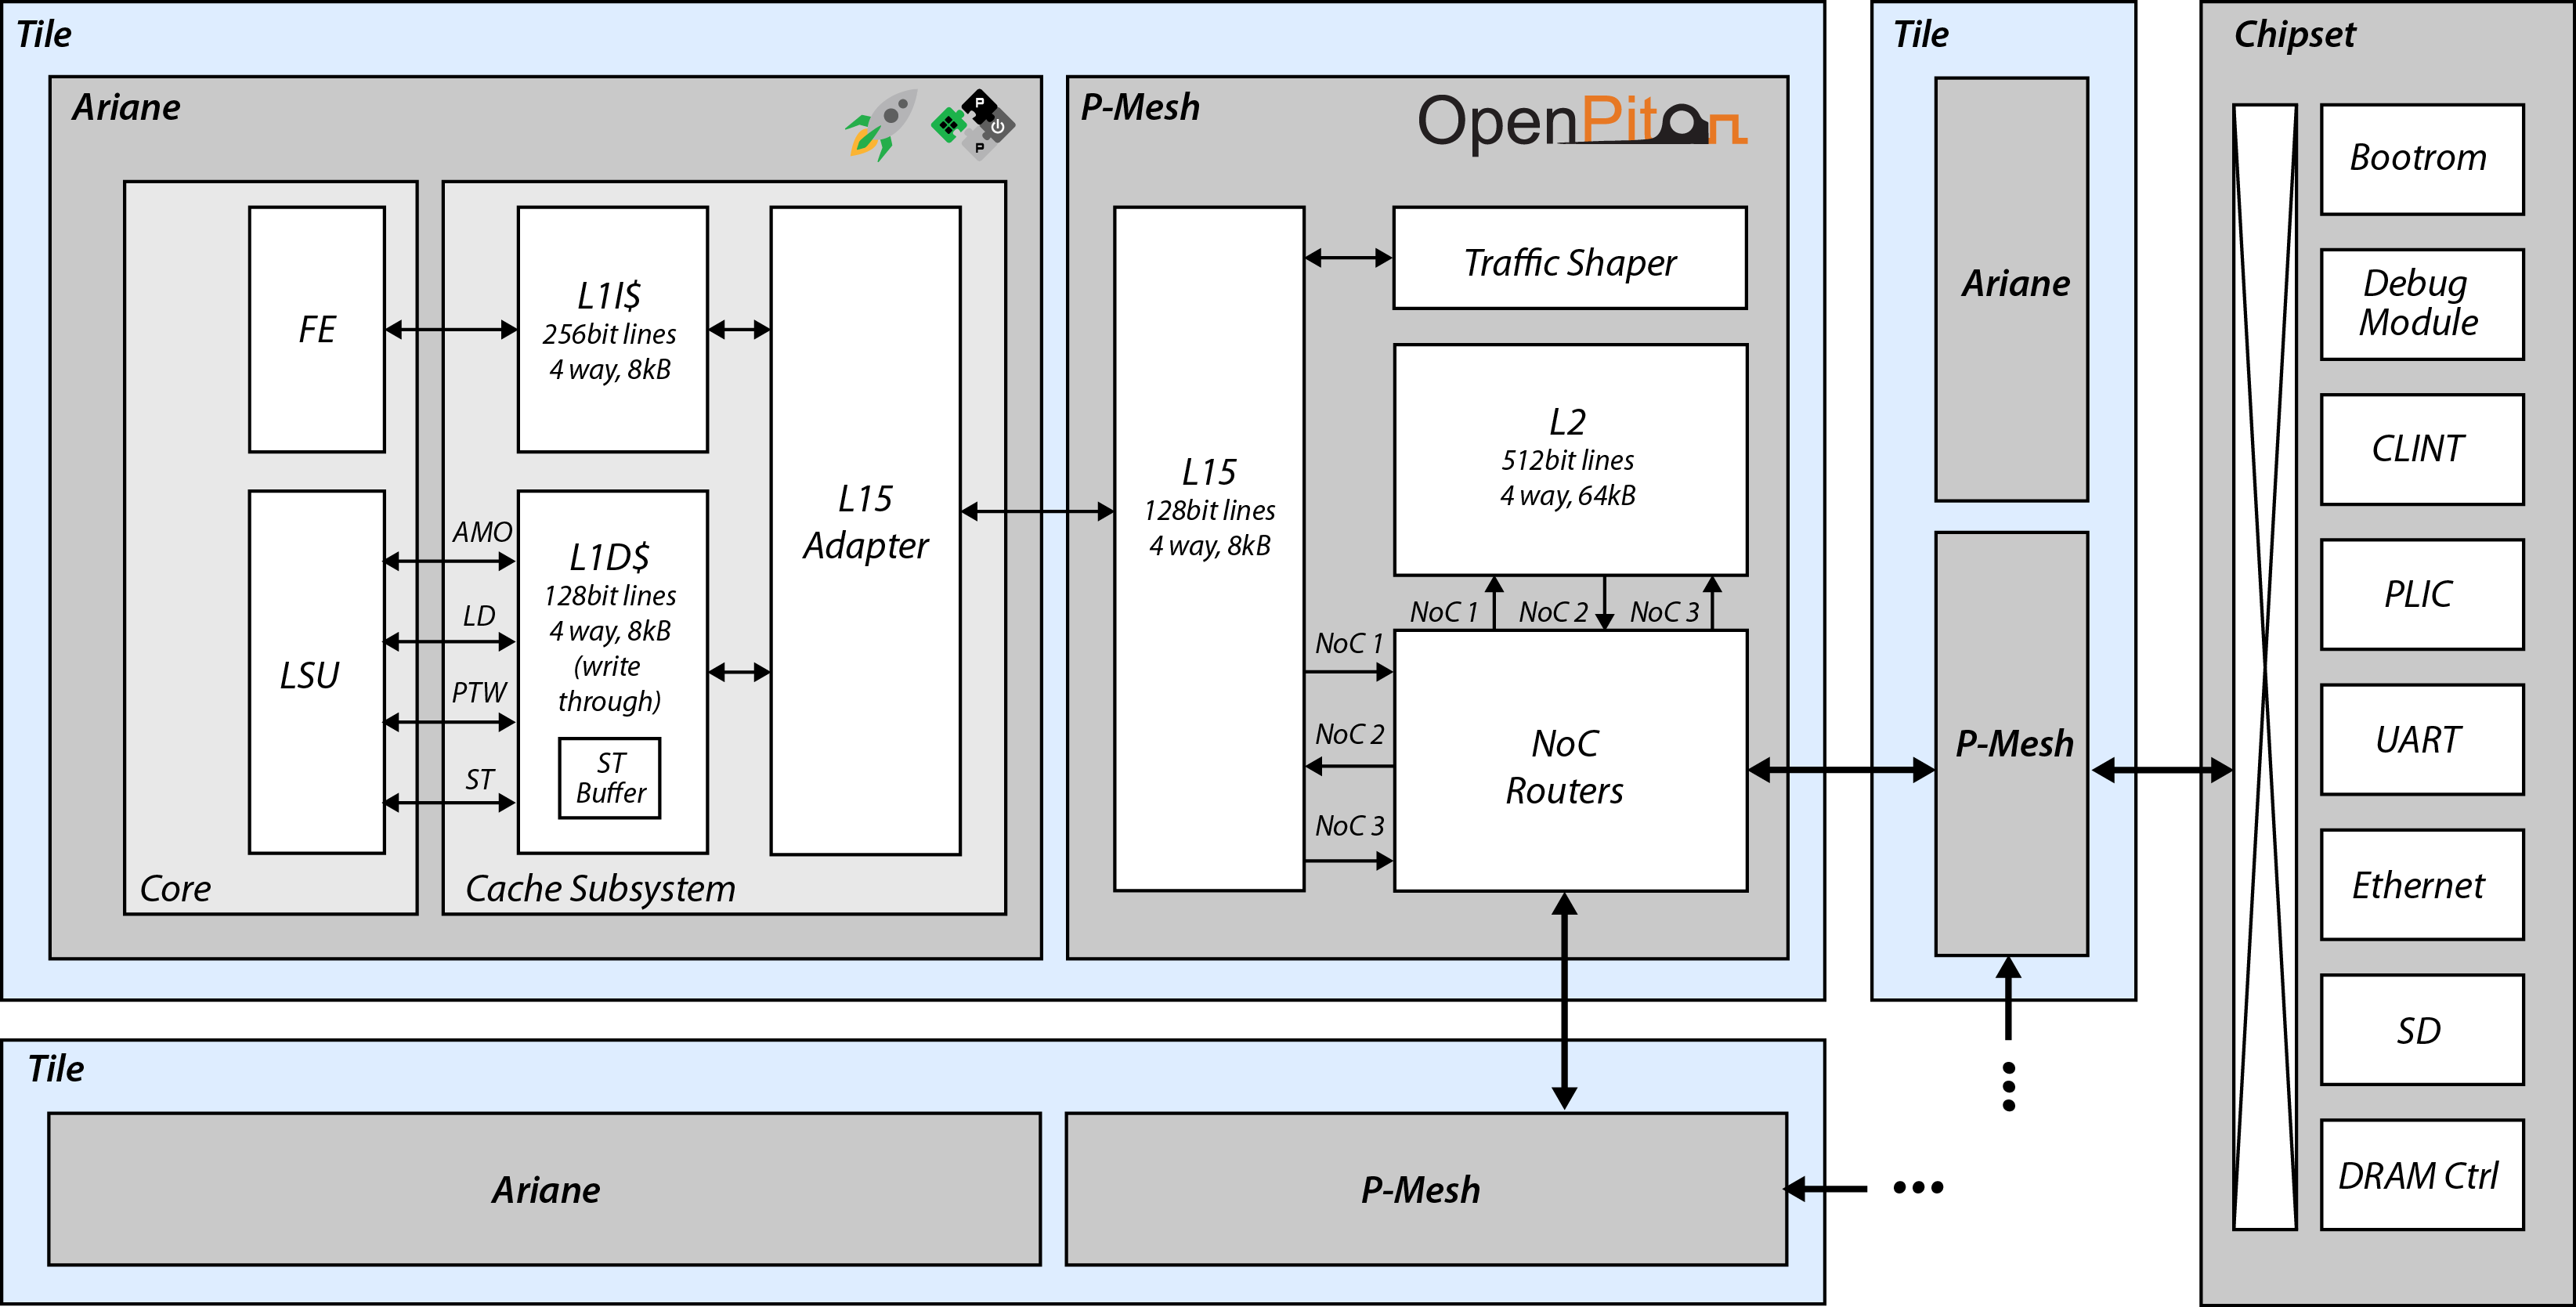
\includegraphics[width=0.9\textwidth]{img/openpiton_ariane_blockdiag.png}
    \caption{Openpiton and ariane block diagram.}
    \label{fig:openpitonariane}
\end{figure}

The main issue we encountered when trying to deploy the core was generating the bitstream. The design only officially supports the "Genesys2", "Nexys Video", and "VC707" boards. We tried to port and adapt it to our board, but we could not manage to do it. We decided to try another core because of the considerable complexity of the project and the knowledge needed to make the portability to our board possible.

\subsection{Rocketchip}
Rocketchip is a \gls{soc} generator designed at the University of Berkeley, California \cite{rocket}. From a configuration, it generates the full implementation, including multiple cores, caches and coherence protocol. It uses Chisel\footnote{\url{https://github.com/chipsalliance/chisel3}} as \gls{hdl}, a Scala-based language for \gls{asic} and \gls{fpga} logic designs. It implements the RISCV64G \gls{isa} variant. It is capable of booting Linux and allow different multicore configurations.

Figure \ref{fig:rocketstruct} shows \gls{soc} structure. The Rocketchip uses Rocket, BOOM or Zscale cores as a basic unit. Each core has its L1 data and instruction caches and a RoCC coprocessor. These units (Tiles) are interconnected using Tilelink, which interconnects the tiles with the level two cache. Tilelink is flexible and allows different cache coherence protocols. Finally, an AXI4 bridge connects the Tilelink module with the AXI4 crossbar, enabling the cores to access various devices and peripherals such as the \gls{dram}, IO devices.

\begin{figure}[h]
  \centering
  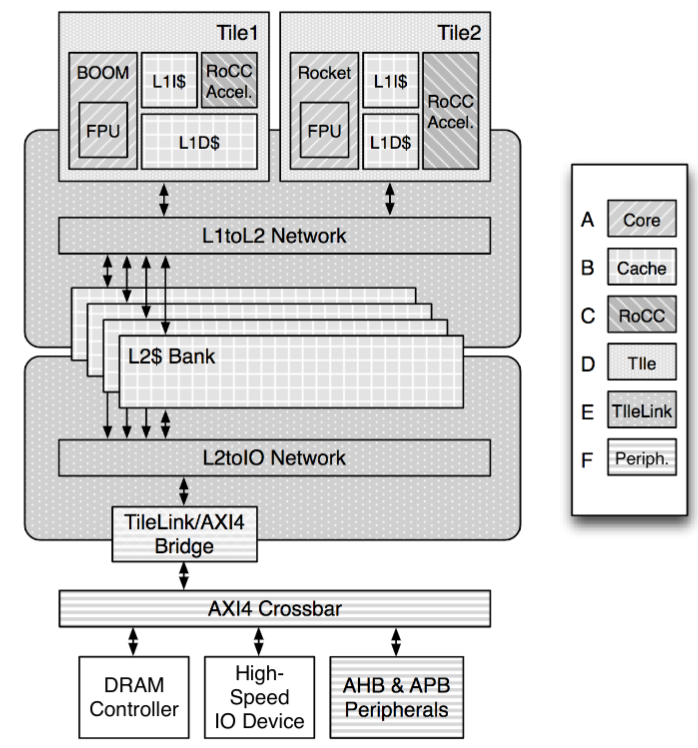
\includegraphics[width=0.6\textwidth]{images/rocket_structure.png}
  \caption{Rocketchip \gls{soc} structure}
  \label{fig:rocketstruct}
\end{figure}

When trying to deploy the Rocketchip \gls{soc}, we found out many difficulties. In particular, the lack of documentation, the Scala-based configuration and the resource usage made the deployment impossible.

\subsection{Darkriscv}
From the previous experience, we decided to take a different approach. We looked for a core that seems simple to deploy to our board and understand and then make the necessary modifications to accomplish project objectives.

Darkriscv\footnote{\url{https://github.com/darklife/darkriscv}} is a tiny and naive core that implements most of the RISCV32E and RISCV32I extensions. It uses few \gls{fpga} resources, and it has been tested on similar \gls{fpga} boards. The core is not designed to be multicore either to boot Linux. Therefore, we decided to rephrase the project objectives and defined new ones. First, to deploy Darkriscv into our \gls{fpga}, modify the design to be multicore capable, including a simple coherence system and boot simple programs to test the multicore design.

Its simplicity makes the design easy to understand, which enabled us to make the necessary modifications towards generating a bitstream for our \gls{fpga}.

Figure \ref{fig:bitstream_gen} illustrates the bitstream generation process. 
First, we create the Vivado project and import the source code files of Darkrsicv. Then we generate the constraints file, which maps between the hardware physical inputs and outputs to logical inputs and outputs for our code. In addition, we create the block design. Figure \ref{fig:block_design} shows the structure. We placed two blocks, a Xilinx Clock IP for our board and the Darksoc block, which contains the core. Then we connected the Xilinx clock to the Darksoc clock, the physical reset button to the core reset, the core LEDs to the board physical LEDs and the system clock to the Xilinx clocking IP.

\begin{figure}[h]
    \centering
    \begin{tikzpicture}[node distance=0.4cm]
      \node (prj) [stylepop] {Create Vivado project};
      \node (const) [stylepop, right=of prj ] {Design constraints file};
      \node (blk) [stylepop, right=of const] {Block design};
      \node (bit) [stylepop, right=of blk] {Generate bitstream};

      \draw [arrow] (prj) -- (const);
      \draw [arrow] (const) -- (blk);
      \draw [arrow] (blk) -- (bit);
    \end{tikzpicture}
    \caption{Bitstream generation process}
    \label{fig:bitstream_gen}
\end{figure}

\begin{figure}[h]
  \centering
  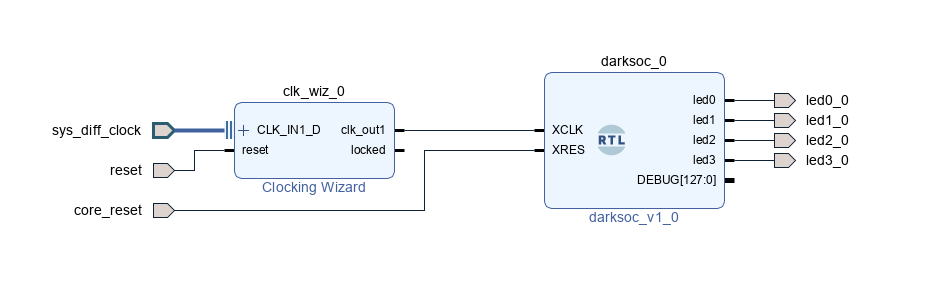
\includegraphics[width=0.8\textwidth]{../presentation/images/block-design.png}
  \caption{Darkriscv block design}
  \label{fig:block_design}
\end{figure}

Finally, once we have the block design, we are capable of synthesizing and generating the bitstream. 

\iffalse
[1] http://parallel.princeton.edu/openpiton/paper.html
[2] https://github.com/PrincetonUniversity/openpiton/blob/openpiton/docs/openpiton_ariane_blockdiag.png?raw=true
[3] https://www2.eecs.berkeley.edu/Pubs/TechRpts/2016/EECS-2016-17.html
[4] https://github.com/chipsalliance/chisel3
[5] Slides
[6] Slides

\fi

\section{Referee}

\begin{frame}{Memory Referee}
\begin{itemize}
    \item Interface between multiple cores and the memory
    \item Forwards single petitions to the memory
    \item Controls the halt of the cores trying to access memory
    \item Scalable to any number of cores
\end{itemize}
\begin{figure}
    \centering
    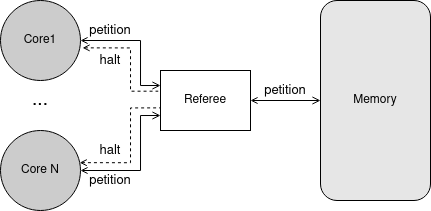
\includegraphics[width=6cm]{images/Referee_fig.png}
    %\caption{Caption}
    \label{fig:my_label}
\end{figure}
\end{frame}

% \begin{frame}{Memory Referee: Ports}
%   \begin{columns}[T]
%     \begin{column}{0.5\textwidth}
%     \textbf{Inputs:}\\
%         From cores:
%         \begin{itemize}
%             \item WR[ncores][1]
%             \item RD[ncores][1]
%             \item DADDR[ncores][32]
%             \item ST\_DATA[ncores][32]
%             \item BE[ncores][4]
%         \end{itemize}
%         From the memory
%         \begin{itemize}
%             \item MEM\_READY[1]
%             \item MEM\_VALID[1]
%             \item MEM\_LD\_DATA[32]
%         \end{itemize}
%     \end{column}
%     \begin{column}{0.5\textwidth}
%     \textbf{Outputs:}\\
%     To the cores
%     \begin{itemize}
%         \item HLT[ncores][1]
%         \item LD\_DATA[1]
%     \end{itemize}
%     To the memory
%     \begin{itemize}
%             \item M\_WR[1]
%             \item M\_RD[1]
%             \item M\_DADDR[32]
%             \item M\_ST\_DATA[32]
%             \item M\_BE[4]
%     \end{itemize}
%   
%     \end{column}
%  \end{columns}
% \end{frame}


\begin{frame}{Memory Referee: Behaviour}
  At any point:
  \begin{itemize}
      \item $PETITION[0..n]$ $\longleftarrow$ $RD[0..n]$ \hspace{0.2cm}$\mid$\hspace{0.2cm} $WR[0..n]$
      
      
      \item $HLT[0..n]$ $\longleftarrow$  $PETITION[0..n]$ \hspace{0.2cm}\&\hspace{0.2cm} $!RELEASE[0..n]$
  \end{itemize}
  
  \begin{columns}[T]
    \begin{column}{0.33\textwidth}
      \textbf{IDLE:}\\
      if $p>0$ petitions from the cores occur:
      \begin{enumerate}
          \item Select one $p_i$.
          \item Send $p_i$ to the main memory.
          \item Transition into WAITING.
      \end{enumerate}
    \end{column}
    \begin{column}{0.33\textwidth}
      \textbf{WAIT\_DATA:}\\
      %Ignore all petitions.\\
      if $mem.valid==1$:
      \begin{enumerate}
          \item $RELEASE[i]=1$
          \item Transition into WAIT\_CORE
      \end{enumerate}
    \end{column}
    \begin{column}{0.33\textwidth}
      \textbf{WAIT\_CORE:}\\
      %Ignore all petitions.
      \begin{enumerate}
          \item $RELEASE[i]=0$
          \item Transition into IDLE
      \end{enumerate}
    \end{column}
  \end{columns}
\end{frame}

\begin{frame}{How to test it}
\begin{columns}[T]
    \begin{column}{0.4\textwidth}
	\textbf{Assembly inline}
    \end{column}
    \begin{column}{0.3\textwidth}
	\textbf{OBJDUMP}
    \end{column}
    \begin{column}{0.1\textwidth}
	\textbf{Hexfile}
    \end{column}
\end{columns}
\vspace{-0.5cm}
\begin{figure}
    \centering
    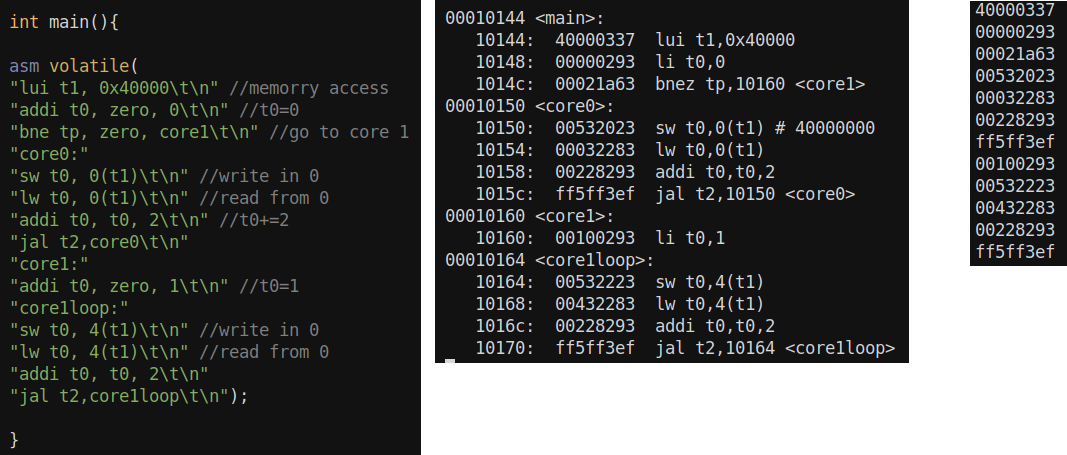
\includegraphics[width=11cm]{images/coding.png}
    %\caption{Caption}
    \label{fig:my_label}
\end{figure}


\end{frame}


\begin{frame}{FLAG test with two cores}
leds=[0 0 0 0], flag0=0, flag1=0.
  \begin{columns}[T]
    \begin{column}{0.4\textwidth}
        \textbf{Core0}\\
        while(1)\{\\
        \hspace{1cm}leds = [0 0 0 1];\\
        \hspace{1cm}flag0 = 1;\\
        \hspace{1cm}while(!flag1);\\
        \hspace{1cm}flag1 = 0;\\
        \hspace{1cm}leds = [0 1 0 0];\\
        \}
    \end{column}
    \begin{column}{0.4\textwidth}
        \textbf{Core1}\\
        while(1)\{\\
        \hspace{1cm}while(!flag0);\\
        \hspace{1cm}flag0 = 0;\\
        \hspace{1cm}leds = [0 0 1 0];\\
        \hspace{1cm}flag1 = 1;\\
        \}
    \end{column}
 \end{columns}
 \begin{figure}
    \centering
    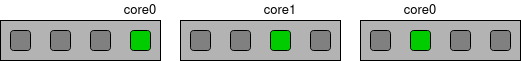
\includegraphics[width=8cm]{images/leds2_fig.png}
    %\caption{Caption}
    \label{fig:my_label}
\end{figure}
\end{frame}

%\begin{frame}{FLAG test with two cores: Simulation}
%\begin{figure}
%    \centering
%    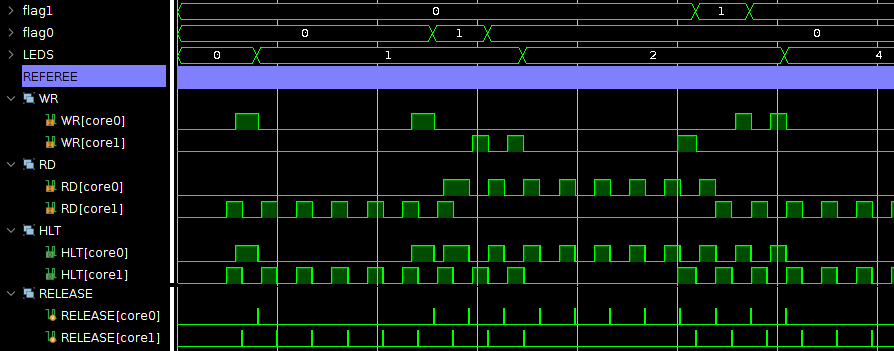
\includegraphics[width=11cm]{images/flag2_sim_crop.png}
%    %\caption{Caption}
%    \label{fig:my_label}
%\end{figure}
%\end{frame}
%
%\begin{frame}{FLAG test with two cores: Simulation}
%\begin{figure}
%    \centering
%    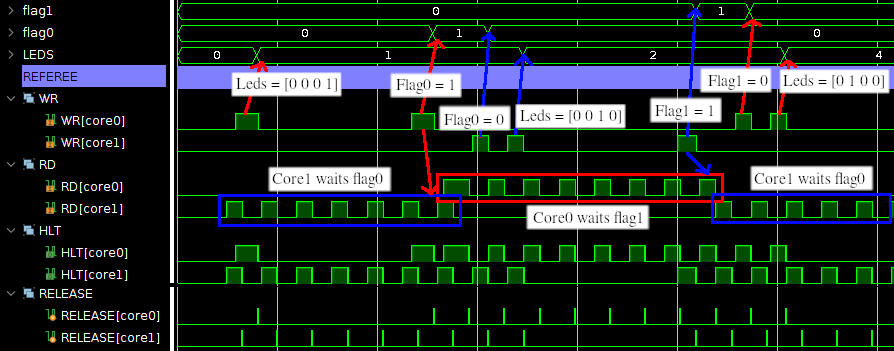
\includegraphics[width=11cm]{images/flag2_sim_crop_arrows.png}
%    %\caption{Caption}
%    \label{fig:my_label}
%\end{figure}
%\end{frame}

% \begin{frame}{FLAG test with two cores: Simulation}
% \begin{figure}
%     \centering
%     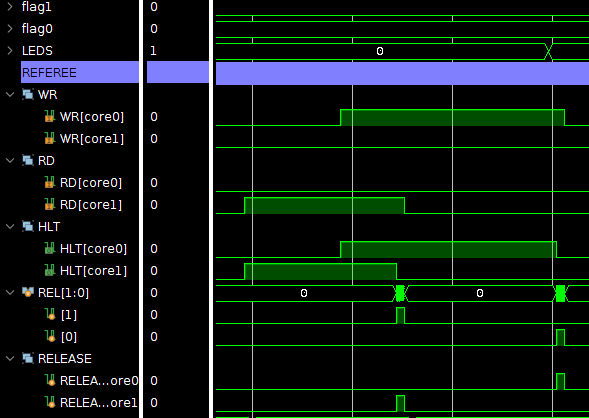
\includegraphics[width=8cm]{images/flag2_sim_close.png}
%     %\caption{Caption}
%     \label{fig:my_label2}
% \end{figure}
% \end{frame}

\begin{frame}{FLAG test with two cores: Simulation}
\begin{figure}
    \centering
    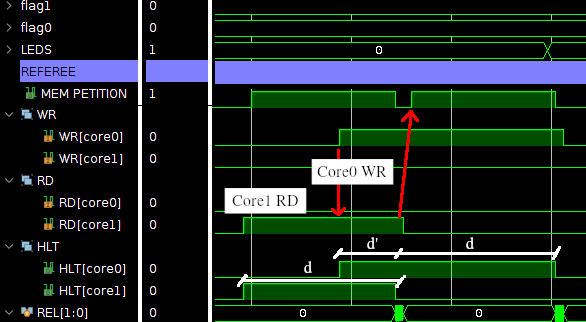
\includegraphics[width=8cm]{images/flag2_sim_close_arrow.png}
    %\caption{Caption}
    \label{fig:my_label2}
\end{figure}
\end{frame}

\begin{frame}{FLAG test with four cores}
  leds=[0 0 0 0], flag=0.
  \begin{columns}[T]
    \begin{column}{0.25\textwidth}
    \textbf{Core0}\\
    while(flag!=0);\\
    leds = [0 0 0 1];\\
    flag = 1;\\
    \end{column}
    \begin{column}{0.25\textwidth}
    \textbf{Core1}\\
    while(flag!=1);\\
    leds = [0 0 1 0];\\
    flag = 2;\\
    \end{column}
    \begin{column}{0.25\textwidth}
    \textbf{Core2}\\
    while(flag!=2);\\
    leds = [0 1 0 0];\\
    flag = 4;\\
    \end{column}
    \begin{column}{0.25\textwidth}
    \textbf{Core3}\\
    while(flag!=4);\\
    leds = [1 0 0 0];\\
    flag = 0;\\
    \end{column}
 \end{columns}
  \begin{figure}
    \centering
    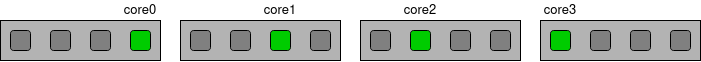
\includegraphics[width=10cm]{images/leds4_fig.png}
    %\caption{Caption}
    \label{fig:my_label}
\end{figure}
\end{frame}

\begin{frame}{FLAG test with four cores: Simulation}
\begin{figure}
    \centering
    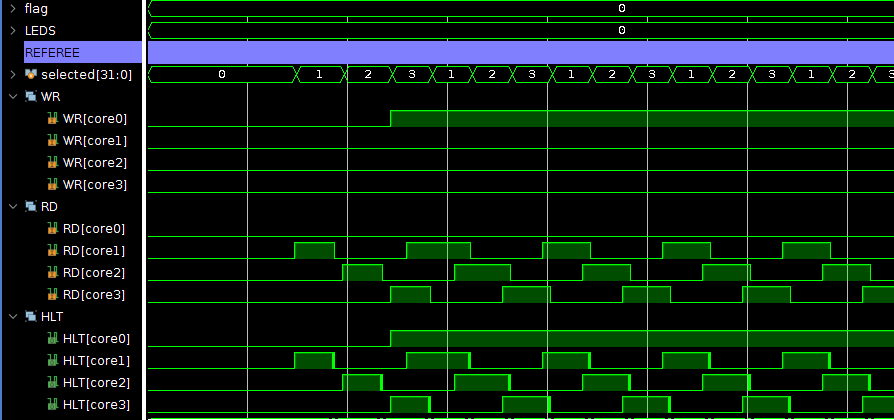
\includegraphics[width=11cm]{images/flag4_sim_bad_crop.png}
    %\caption{Caption}
    \label{fig:my_label}
\end{figure}
\end{frame}

\begin{frame}{FLAG test with four cores: Simulation}
\begin{figure}
    \centering
    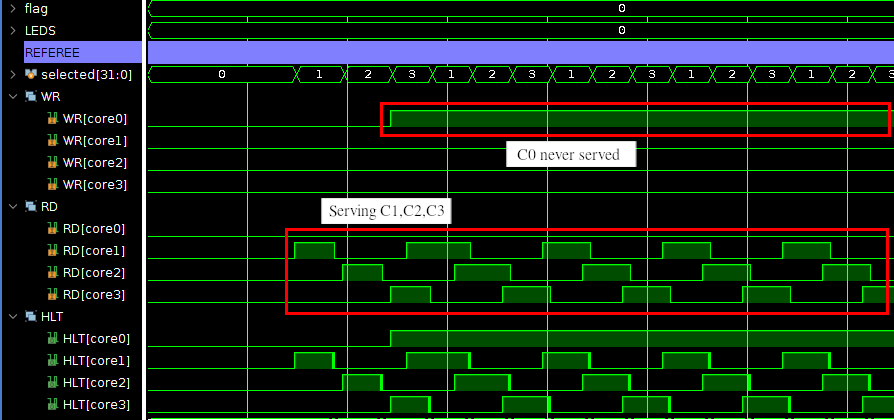
\includegraphics[width=11cm]{images/flag4_sim_bad_crop_arrow.png}
    %\caption{Caption}
    \label{fig:my_label}
\end{figure}
\end{frame}

%\begin{frame}{FLAG test with four cores: Simulation}
%\begin{figure}
%    \centering
%    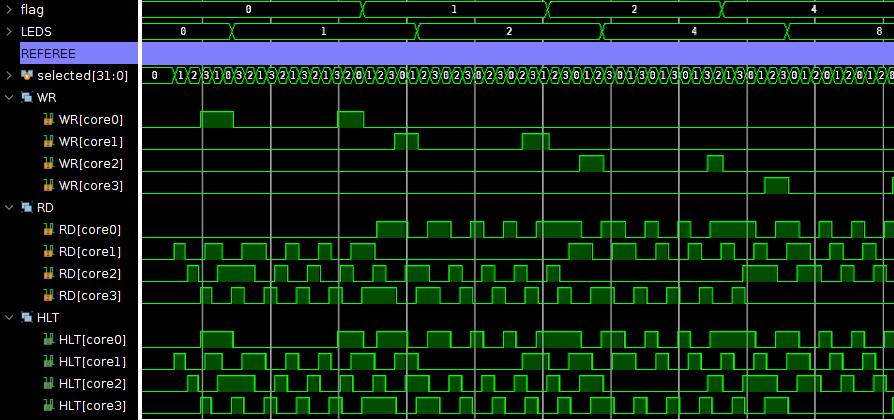
\includegraphics[width=11cm]{images/flag4_sim_good_crop.png}
%    %\caption{Caption}
%    \label{fig:my_label}
%\end{figure}
%\end{frame}

\begin{frame}{Dot product multicore}
Dot product: $\sum_{i=0}^{n}{v_{i} * u_{i}}$
\vspace{0.2cm}
\begin{enumerate}
    \item Barrier after initialization
\end{enumerate}
\begin{figure}
    \centering
    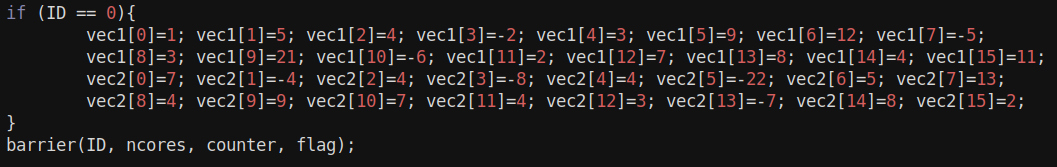
\includegraphics[width=11cm]{images/axpy_ini.png}
    \label{fig:my_label}
\end{figure}

\begin{enumerate}
    \item Reduction of the result
\end{enumerate}
\begin{figure}
    \centering
    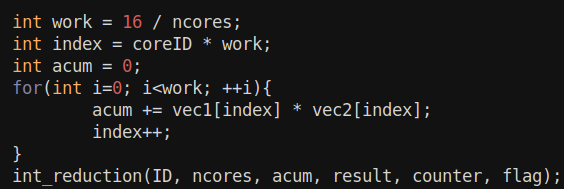
\includegraphics[width=6cm]{images/axpy_body.png}
    \label{fig:my_label}
\end{figure}


\end{frame}

\begin{frame}{Dot product with 4 cores: Simulation}
\begin{figure}
    \centering
    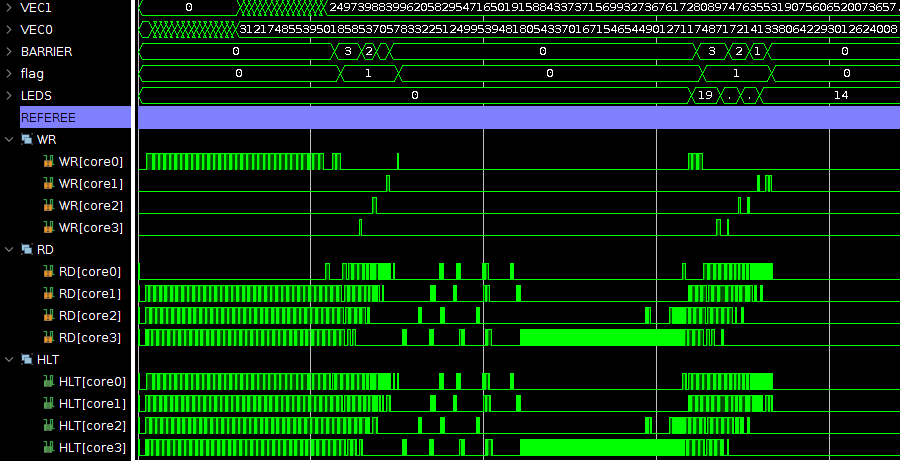
\includegraphics[width=11cm]{images/axpy_sim4_crop.png}
    %\caption{Caption}
    \label{fig:my_label}
\end{figure}
\end{frame}

\begin{frame}{Dot product with 4 cores: Simulation}
\begin{figure}
    \centering
    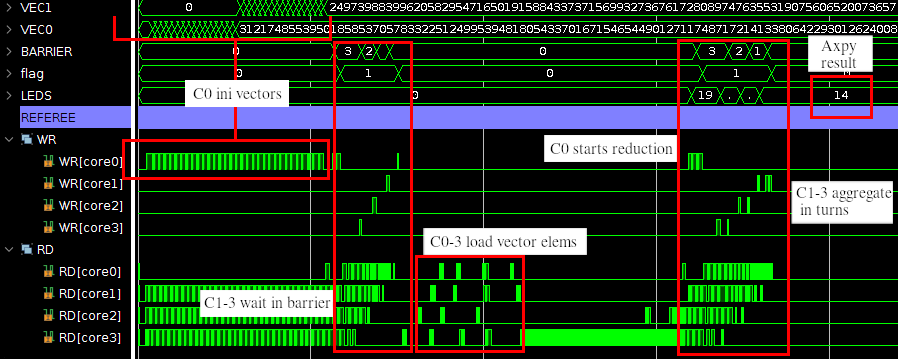
\includegraphics[width=11cm]{images/axpy_sim4_crop_arrow.png}
    %\caption{Caption}
    \label{fig:my_label}
\end{figure}
\end{frame}

\begin{frame}{Dot product with 8 cores: Simulation}
\begin{figure}
    \centering
    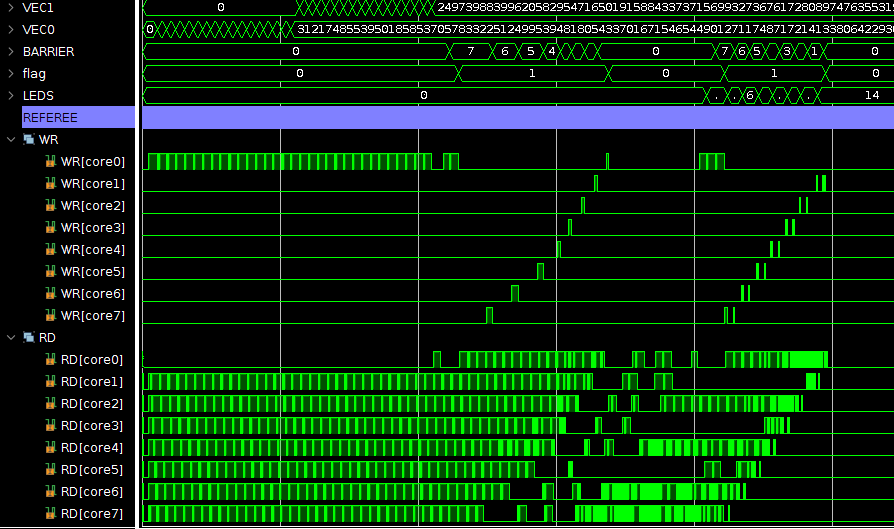
\includegraphics[width=11cm]{images/axpy_sim8_crop.png}
    %\caption{Caption}
    \label{fig:my_label}
\end{figure}
\end{frame}


\section*{}

\begin{frame}[allowframebreaks]
        \frametitle{References}
\bibliographystyle{unsrt}
\bibliography{../common/99_ref}
\end{frame}


\begin{frame}{}
    \centering
    \Large Thanks for your attention.
\end{frame}

\end{document}
